\section{Introduction}
\label{sec:intro}
Visual SLAM is a fundamental problem in 3D computer vision, with wide applications in autonomous driving, robotics, virtual reality, and augmented reality. SLAM aims to construct dense or sparse maps to represents the scene. Recently, neural rendering \cite{NeRF2020} has been integrated into SLAM pipelines, significantly enhancing the scene representation capabilities of the maps. The latest advancement in radiance field rendering is 3D Gaussian Splatting (3DGS) \cite{3DGS2023}, an explicit scene representation that achieves revolutionary improvements in rendering and training speed. Recent SLAM works \cite{Photo-SLAM2024, MonoGS2024, SplaTAM2024, GS-SLAM2024, RTG-SLAM2024, CG-SLAM2024, GS-ICPSLAM2024} incorporating 3DGS have demonstrated that explicit representations provide more promising rendering performance compared to implicit representations.

%然而当前的采用3DGS的SLAM算法没能同时在单目、双目、以及RGB-D相机上同时取得高质量的渲染结果。目前已有的算法大多仅支持RGB-D。例如,SplaTAM 通过最小化图像和深度重建误差优化3D高斯,实现了对于RGB-D相机的定位与渲染。GS-SLAM 通过RGB-D重渲染损失实现了相机位姿跟踪和稠密建图。RTG-SLAM对于RGB-D相机提出了一种高效的流水线。 GS-ICP SLAM 提出了一种新的表征完成了稠密重建。CG-SLAM基于不确定性启发的3D高斯场,实现了一种高效的RGB-D SLAM。还有一些算法同时支持单目、双目和RGB-D相机。例如,MonGS直接根据3DGS优化实现相机跟踪的推导,同时支持于单目、双目与RGB-D的定位与渲染。但该算法双目与单目之间的渲染质量存在很大的差距。Photo-SLAM 提出了一种解耦的框架来优化3D高斯,实现了对于单目、双目与RGB-D的实时定位与渲染。其具有优秀的实时性,并且单目与RGB-D相机的渲染结果差距很小,但是其总体渲染质量仍然较差。

However, current SLAM methods leveraging 3DGS have yet to achieve high-quality rendering across monocular, stereo, and RGB-D cameras simultaneously. Most existing approaches only support RGB-D cameras. For example, SplaTAM \cite{SplaTAM2024} jointly optimizes the camera pose and the Gaussians by minimizing the image and depth reconstruction errors, achieving localization and rendering for RGB-D cameras. GS-SLAM \cite{GS-SLAM2024} derives an analytical formulation for optimizing camera pose tracking and dense mapping with RGB-D re-rendering loss. RTG-SLAM \cite{RTG-SLAM2024} proposes a efficient pipeline to derive a compact Gaussian representation, resulting a real-time RGB-D system. GS-ICP SLAM \cite{GS-ICPSLAM2024} propose a novel dense RGB-D SLAM approach with a fusion of Generalized Iterative Closest Point (ICP) and 3DGS. CG-SLAM \cite{CG-SLAM2024} employs an uncertainty-aware 3D Gaussian field to achieve efficient RGB-D SLAM. 

There are a few methods supporting monocular, stereo, and RGB-D cameras. MonGS \cite{MonoGS2024} formulates camera tracking for 3DGS using direct optimization against the 3D Gaussians, allowing localization and photorealistic mapping for all three types of cameras. Unfortunately, its rendering quality gap between stereo and monocular cameras is significant. Photo-SLAM \cite{Photo-SLAM2024} introduces a decoupled framework to optimize 3D Gaussians, achieving real-time localization and photorealistic mapping for monocular, stereo, and RGB-D cameras. While it demonstrates strong real-time performance and a minimal gap in rendering quality between monocular and RGB-D cameras, its primary  limitation lies in the overall rendering quality. Our work aims to significantly improve the rendering accuracy for monocular, stereo, and RGB-D cameras.

In this paper, we propose \emph{Scaffold}-SLAM, a novel SLAM system that achieves simultaneous localization and high-quality photorealistic mapping across monocular, stereo, and RGB-D cameras. Our approach shares the same decoupled framework as Photo-SLAM \cite{Photo-SLAM2024}, where we utilize a traditional indirect visual SLAM pipeline for localization and geometric mapping. The generated point cloud is used to initialize structured 3D Gaussians. Instead, we introduce two key innovations that enable our method to achieve state-of-the-art photorealistic mapping quality across monocular, stereo, and RGB-D cameras. First, we propose Appearance-from-Motion embedding, which models appearance variations such as exposure and lighting in a learned low-dimensional latent space. We train the embedding to predict the appearance variations across diverse images with the camera pose. Second, we propose a frequency regularization pyramid that constrains the frequencies of rendered image across multiple scales in the frequencies domain. This encourages 3D Gaussians to grow towards complex regions, such as object edges and textures, enabling the model to capture high-frequency details in the scene. Finally, to evaluate the photorealistic mapping quality of our method, we conduct extensive experiments across diverse datasets, including monocular, stereo, and RGB-D cameras. The experimental results show that our approach, \emph{Scaffold}-SLAM, surpasses state-of-the-art methods in photorealistic mapping quality across all three camera types. The main contributions of this work are as follows:
\begin{enumerate}
    \item We develop an Appearance-from-Motion embedding to enable our SLAM system to effectively model image appearance variations across diverse images.
    \item We propose a frequency regularization pyramid  to guide the growth
    of 3D gaussians toward complex regions to capture finer details in the scene.
    \item Extensive evaluations on various datasets demonstrate that our method, \emph{Scaffold}-SLAM, achieves superior photorealistic mapping quality across monocular, stereo, and RGB-D cameras, while maintaining competitive tracking accuracy. The code will be publicly available.
\end{enumerate}

\begin{figure*}[t]
  \centering
   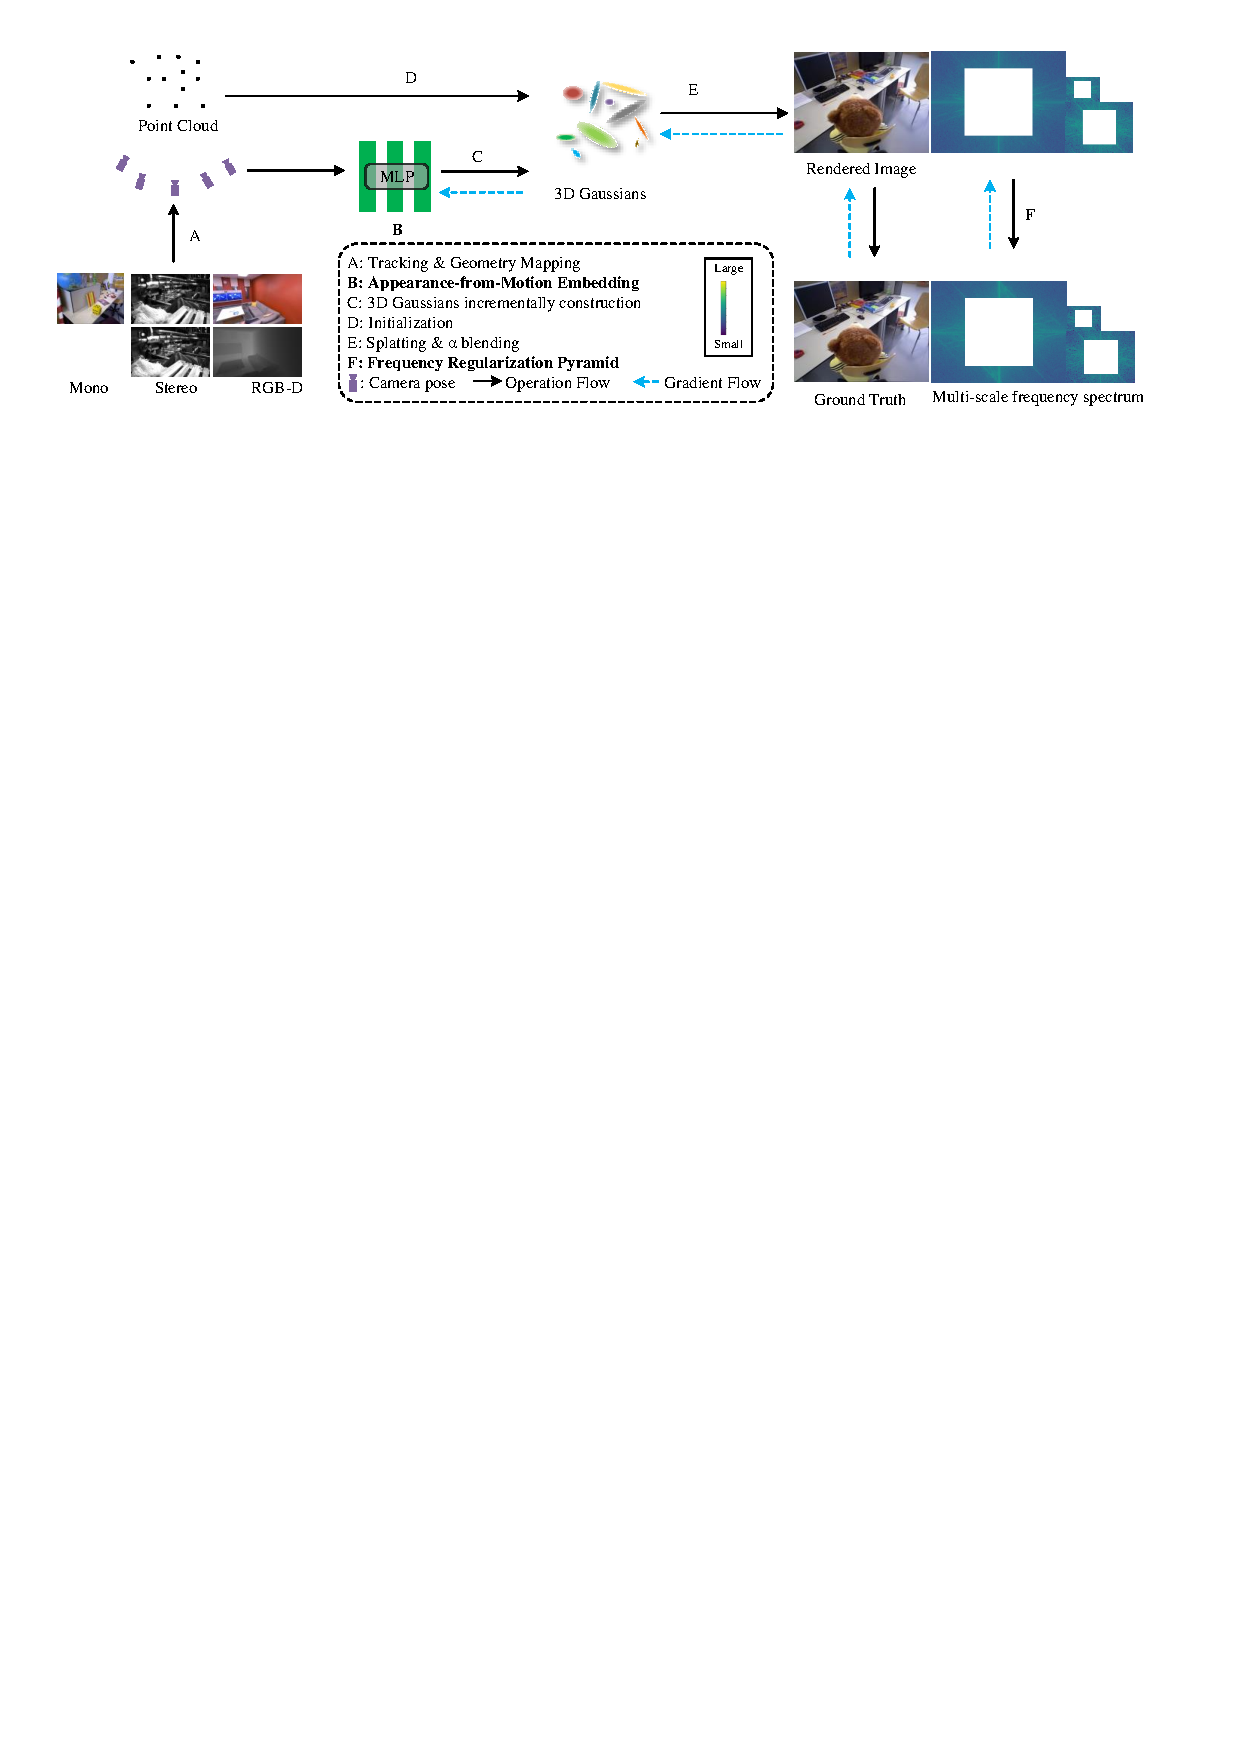
\includegraphics[width=1\linewidth]{fig/diagram.pdf}
   \caption{Overview of our method. Our method supports monocular, stereo, and RGB-D cameras. The input image stream is processed by the tracking and geometric mapping modules, generating high-quality point cloud and accurate poses. These point cloud are used to incrementally construct Gaussians. The poses are fed into the Appearance-from-Motion embedding to model lighting and other appearance changes in the environment. Additionally, we introduce the frequency regularization pyramid to supervise the training of Gaussians, allowing for improved modeling of high-frequency details in the scene.}
   \label{fig:diagram}
\end{figure*}
\section{Related Work}
\label{sec:intro}

\noindent\textbf{Visual SLAM.} Traditional visual SLAM methods can be broadly classified into two categories: direct methods and indirect methods. Indirect methods rely on extracting and tracking features between consecutive frames to estimate pose and build sparse maps by minimizing the reprojection error. Examples include PTAM \cite{PTAM}  and ORB-SLAM3 \cite{ORB-SLAM32021}. Direct methods \cite{LSD-SLAM, DSO, DSM}, on the other hand, bypass feature extraction and estimate motion and structure by minimizing photometric error, which can build sparse or semi-dense maps. The first dense visual SLAM is KinectFusion \cite{KinectFusion}, which updates the scene using a TSDF representation. Recently, some methods \cite{CodeSLAM, SceneCode, NodeSLAM, DROID-SLAM2021, MS_SLAM_2024CVPR} have integrated deep learning into visual SLAM systems. DPVO \cite{DPVO} extends the current state-of-the-art method Droid-SLAM \cite{DROID-SLAM2021} by leveraging the efficiency of sparse block matching, improving computational performance. More recently, Lipson et al. \cite{MS_SLAM_2024CVPR} couple optical flow prediction with a pose-solving layer to achieve camera tracking.  Our approach favors traditional indirect SLAM for the following insight. Indirect SLAM shares a highly similar pipeline with Structure-from-Motion (SfM), including feature matching, tracking, and bundle adjustment, leading to point cloud with similar intrinsic properties. Since the 3D Gaussians in \cite{3DGS2023}  are initialized by point cloud generated frome SfM, we believe that initializing our Gaussians using point cloud obtained from indirect SLAM is an optimal choice.
%这段可以精简
%传统的视觉SLAM主要包含直接法和间接法两大类。间接法通过提取和跟踪连续帧之间的特征,根据最小化重投影误差完成定位与稀疏建图。例如,PTAM, ORB-SLAM3。直接法则不提取特征,而是通过最小化一个光度误差来估计位姿与环境结构。例如,LSD-SLAM,DSO,DSM, 他们能构建一个稀疏或半稠密地图。 KinectFusion 不属于这两类,它通过对RGB-D采集的深度点云执行ICP实现跟踪,通过TSDF更新场景,是第一个稠密的视觉SLAM。最近,一些方法将深度学习引入视觉SLAM系统,例如CodeSLAM, SceneCode, NodeSLAM 和Droid-SLAM。Droid-SLAM是目前的SOTA,提出了一种dense BA layer来实现定位与稠密建图。它在一个庞大的数据集TartanAir训练它的模型。DPVO 是 Droid-SLAM的扩展,利用了基于稀疏块匹配的优势,提升了效率性。Deng 等人提出一种端到端方法,耦合光流预测和求解层来实现相机位姿跟踪,是该领域的最新进展。我们采用传统间接法SLAM的见解是,间接法SLAM与SfM具有高度相似的pipline,均包含特征匹配与跟踪,BA。他们生成的点云具有相似的内在性质。3DGS采用SfM生成的点云来初始化3DGS,因此我们认为采用间接法得到的点云来初始化我们的高斯是一种更优的选择。
%可以分类为稀疏SLAM和稠密SLAM。其中稀疏SLAM首先匹配图像之间的特征点,通过最小化重投影误差实现跟踪和建图,例如PTAM,ORB-SLAM3。由于特征点比较稀疏,其获得的地图通常比较稀疏。但这类方法通常具备很高的鲁棒性。稠密SLAM能构建相当稠密的环境地图,实现场景的重建。一些直接手工的方法能完成这个任务。例如DTAM基于图像之间光度的一致性来跟踪与将场景表示成体积。KinectFusion 通过ICP实现跟踪,通过TSDF更新场景。最近一些方法将深度学习引入SLAM框架中,实现了更精确的定位与建图,例如Droid-SLAM,CodeSLAM。SceneCode,and NodeSLAM.


%首先将辐射场渲染引入SLAM系统中的是神经隐式表征。iMAP首先引入神经隐式表征,根据重建误差实现跟踪与建图 随后许多工作探索了新的表征形式。NICE-SLAM在iMAP的基础上引入了多层特征栅格,具备构建更大场景的能力。Vox-Fusion proposed a voxel-based neural implicit surface representation to encode the scene. Orbeez-SLAM combine InstantNGP with ORB-SLAM, resulting a reat-time neural dense SLAM system. ESLAM represent scene as multi-scale axis-aligned perpendicular feature planes, resulting a efficient system. Co-SLAM is a RGBD-SLAM system which represents the scene as a multi-resolution hash-grid. SNI-SLAM introduce hierarchical semantic representation to performs accurate semantic mapping high-quality surface reconstruction and robust camera tracking. NGEL-SLAM use octree-based implicit representations to ensure global consistency and low latency. IBD-SLAM propose a xyz-map representation based on an image-based depth fusion model to achieve generalizable SLAM. 一些工作也对其他问题进行了探索。例如,GO-SLAM 将神经隐式表征引入Dorid-SLAM,实现了对于单目、双目以及RGB-D相机的跟踪与重建。Loopy-SLAM is a neural RGBD SLAM system with a novel loop closure by performing global place recognition. PLGSLAM proposes a progressive scene representation method to achieve real-time surface reconstruction and robust camera tracking in large scenarios. 但这些工作都侧重与场景几何结构重建,没有关注新视角图像的渲染质量。Point-SLAM采用了一种基于点的神经隐式表征,通过执行体渲染实现了远超之前方法的渲染效果。 然而,最近的一些方法MonoGS、photo-SLAM证明引入3DGS的的SLAM比Point-SLAM具有更高的渲染精度与速度。


%CP-SLAM presents a complete SLAM system with odometry, loop detection, sub-map fusion, and global refinement. UncLe-SLAM present an uncertainty learning framework for dense neural SLAM with an online sensor uncertainty estimation module. HI-SLAM employ multi-resolution grid encoding and signed distance function (SDF) representation. NICER-SLAM, a dense RGB SLAM system that simultaneously optimizes for camera poses and a hierarchical neural implicit map representation. NIS-SLAM, an efficient neural implicit semantic RGB-D SLAM system, that leverages a pre-trained 2D segmentation network to learn consistent semantic representations. Co-SLAM \cite{Co-SLAM2023} is an RGB-D SLAM system that represents the scene as a multi-resolution hash-grid.

\noindent\textbf{Implicit Representation based SLAM.} 
The first to introduce radiance field rendering into SLAM systems is neural implicit representations. iMAP \cite{iMAP2021} pioneers the use of neural implicit representations to achieve tracking and mapping through reconstruction error. Subsequently, many works \cite{NICE-SLAM2022, Vox-Fusion2022, Orbeez-SLAM2023, ESLAM2023,Co-SLAM2023, SNI-SLAM2024, NGEL-SLAM2024,IBD-SLAM_2024_CVPR,NICER-SLAM2024} have explored new representation forms. For instance, Vox-Fusion \cite{Vox-Fusion2022} proposes a voxel-based neural implicit surface representation. ESLAM \cite{ESLAM2023} represents scenes using multi-scale axis-aligned perpendicular feature planes.  Point-SLAM \cite{Point-SLAM2023} adopts a point-based neural implicit representation and achieved far superior rendering quality compared to previous methods. Recently, SNI-SLAM \cite{SNI-SLAM2024} and IBD-SLAM \cite{IBD-SLAM_2024_CVPR} introduce a hierarchical semantic representation and an xyz-map representation, respectively. Some works \cite{GO-SLAM2023, Loopy-SLAM2024, PLGSLAM_2024_CVPR, CP-SLAM2023, UncLe-SLAM2023, HI-SLAM2024_NeRF, NIS-SLAM2024}  have investigated other challenges. GO-SLAM \cite{GO-SLAM2023} integrates Droid-SLAM, while Loopy-SLAM \cite{Loopy-SLAM2024} addresses loop closure. However, only Point-SLAM explores novel view synthesis, while others focus on geometric reconstruction.

%最近,一些工作将一种显示的表征形式,3DGS,引入视觉SLAM系统实现了定位与真实感建图。得益于3DGS的快速训练与渲染速度、优秀的渲染的特性,这些工作的结果展现了超越了包括Point-SLAM的众多隐式表征方法的真实感建图质量与渲染速度。在这些工作中,大部分工作为RGB-D SLAM系统。SplaTAM 和 GS-SLAM均通过最小化图像和深度渲染误差,来优化相机位姿与建图。RTG-SLAM 探索了高斯表征的效率性,开发了一种实时的RGB-D SLAM系统。 GS-ICP通过对深度点进行融合3DGS的通用ICP实现了一种高质量的真实感建图系统。CG-SLAM 研究了RGB-D传感器的不确定性。另外一些方法同时支持单目、双目、与RGB-D相机。MonoGS推导了优化3D高斯直接完成位姿估计的公式。但其渲染质量在单目相机上表现很糟糕。Photo-SLAM 提出了一种实时的、解耦的定位与真实感建图系统。其优点在于惊人实时性与的资源消耗,但缺点在于其牺牲了太多的渲染质量。我们提出的系统旨在实现对于单目、双目与RGB-D相机的更高质量的真实感建图与具有竞争力的定位精度。与Photo-SLAM相同,本文方法的特性不包含重建一个稠密的mesh。
%我们的同期工作,OG-Mapping是关注于场景的结构性RGB-D的SLAM。LoopSplat和GLC-SLAM则探索3DGS相关的回环检测。IG-SLAM侧重于单目相机。MGSO和GEVO则研究了效率性。Hi-SLAM则引入了语义信息。

%Hi-SLAM we introduce a novel hierarchical representation that encodes semantic information in a compact form into 3D Gaussian Splatting, leveraging the capabilities of large language models.GEVO achieves comparable map fidelity while reducing the memory overhead to around 58 MBs. MGSO provides dense structured point clouds for 3DGS initialization, accelerating ptimization and producing more efficient maps with fewer Gaussians. GLC-SLAM employs frame-to-model tracking and triggers hierarchical loop closure using a globaltoocal strategy to minimize drift accumulation. OG-Mapping  achieve efficient and robust online dense mapping by leverages the robust scene structural representation capability of sparse octrees IG-SLAM is a dense RGB-only SLAM system that employs robust dense SLAM methods for tracking and combines them with Gaussian Splatting. LoopSplat triggers loop closure online and computes relative loop edge constraints between submaps directly via 3DGS registration, leading to improvements in efficiency and accuracy over traditional global-to-local point cloud registration.


\noindent\textbf{3D Gaussian Splatting based SLAM.} 
Recently, several works have introduced an explicit representation, 3DGS \cite{3DGS2023}, into visual SLAM systems, achieving both localization and photorealistic mapping. Thanks to the fast training and rendering speed of 3DGS, as well as its excellent rendering quality, these methods have demonstrated superior photorealistic mapping quality and rendering speed compared to various implicit representation approaches \cite{NICE-SLAM2022, Vox-Fusion2022, Orbeez-SLAM2023, ESLAM2023,Co-SLAM2023, GO-SLAM2023,Point-SLAM2023}, including Point-SLAM \cite{Point-SLAM2023}. Most of these methods are RGB-D SLAM systems. For example, SplaTAM \cite{SplaTAM2024} and GS-SLAM \cite{GS-SLAM2024} both optimize camera poses and mapping by minimizing image and depth rendering errors. RTG-SLAM \cite{RTG-SLAM2024} explores the efficiency of Gaussian representations. GS-ICP \cite{GS-ICPSLAM2024} achieves high-quality photorealistic mapping by fusing 3DGS with Generalized ICP on depth points. CG-SLAM \cite{CG-SLAM2024} examines the uncertainty in RGB-D sensors. Some methods support monocular, stereo, and RGB-D cameras simultaneously. MonoGS \cite{MonoGS2024} formulates directly estimating camera poses by optimizing 3D Gaussians. However, its rendering quality performs poorly on monocular cameras. Photo-SLAM \cite{Photo-SLAM2024} proposes a real-time, decoupled system for localization and photorealistic mapping. Photo-SLAM excels in impressive real-time performance and resource efficiency, but at the cost of significantly reduced rendering quality. Our proposed \emph{Scaffold}-SLAM aims to achieve higher-quality photorealistic mapping for monocular, stereo, and RGB-D cameras while maintaining competitive localization accuracy. Similar to Photo-SLAM, our method does not involve reconstructing a dense mesh.

In concurrent works, OG-Mapping \cite{OG-Mapping} is the RGB-D SLAM leveraging scene structure. LoopSplat \cite{LoopSplat} and GLC-SLAM \cite{GLC-SLAM_2409} explore loop closure detection using 3DGS. IG-SLAM \cite{IG-SLAM_202408} specializes in monocular camera. MGSO \cite{MGSO_2409} and GEVO \cite{GEVO2024} investigate efficiency. Hi-SLAM \cite{Hi-SLAM2024_GS} focus on semantic information.
% recent approaches \cite{SplaTAM2024,MonoGS2024,GS-SLAM2024,GS-ICPSLAM2024, Photo-SLAM2024, CG-SLAM2024, RTG-SLAM2024} have shown that incorporating 3DGS into SLAM systems achieves higher rendering quality and speed compared to Point-SLAM.
% %decouple coupled
% SplaTAM \cite{SplaTAM2024} jointly optimizing the camera pose and the Gaussians by minimizing the image and depth reconstruction error. MonoGS \cite{MonoGS2024} formulate camera tracking for 3DGS using direct optimisation against the 3D Gaussians. GS-SLAM \cite{GS-SLAM2024} derive an analytical formulation for optimizing camera pose tracking and dense mapping with RGB-D re-rendering loss.  GS-ICP SLAM \cite{GS-ICPSLAM2024} propose a novel dense representation SLAM approach with a fusion of Generalized Iterative Closest Point and 3DGS. They utilize a single Gaussian map for both tracking and mapping.  Photo-SLAM \cite{Photo-SLAM2024}, a real-time system, tracks the camera pose based on ORB-SLAM3 and photorealistic mapping the scene as 3DGS pipline. There are also works that focus on the accuracy of geometric reconstruction. CG-SLAM \cite{CG-SLAM2024} presents an efficient dense RGB-D SLAM system, based on a novel uncertainty-aware 3D Gaussian field with high consistency and geometric stability.  RTG-SLAM \cite{RTG-SLAM2024} proposes a efficient pipeline to derive a compact Gaussian representation, resulting a real-time 3D
% reconstruction system with an RGBD camera for large-scale environments.
% Among coupled methods, SplaTAM,  MonoGS and GS-SLAM provide better rendering quality, but both training and tracking are time-consuming. GS-ICP SLAM is the only real-time system with high rendering performance. 
% However, the robustness of this method is poor, and its performance will degrade catastrophically in scenarios with substantial noise and uncertainty in the depth images. Photo-SLAM achieves high real-time performance. while suffering from poor rendering quality. 




%视觉SLAM是3DCV中一种基本的问题,在无人驾驶、机器人、VR、AR中均有广泛应用。传统SLAM旨在实现精确的定位与并构建一个稠密/稀疏的地图。最近将神经渲染引入SLAM流水管线,增强地图的场景表征能力。辐射场渲染最新的进步是一种显示的场景表征3DGS,与NeRF相比,其在渲染和训练速度上有了革命性的进步。最近一些结合3DGS的SLAM工作证明了与隐式表征相比,采用显示表征具备更为令人期待的渲染性能。

%结合3DGS的稠密视觉SLAM根据定位与建图关联可以分为两类。第一类是耦合的方法,通过训练的高斯模型,同时迭代优化相机位姿与高斯,包括SplaTAM、MonoGS、GS-SLAM、GS-ICP SLAM等。 这种训练框架通常具备更高的渲染精度,但其缺点在于很慢的训练速度以及很差的定位实时性。

%另一类是解耦的方法,他们将定位与高斯的训练解耦,其定位通常基于传统视觉SLAM(例如ORB-SLAM)或者基于学习的SLAM(deriod-SLAM),其渲染模块则遵从3DGS的管线,代表工作是Photo-SLAM。其定位模块基于ORB-SLAM3,ORB-SLAM3生成的得到的稀疏点云在本质上与SfM生成点云类似,使其天然适合初始化3DGS。得益于3DGS的较快的训练和渲染速度,以及ORB-SLAM3的效率,Photo-SLAM具有很强的实时性。然而,它最大的局限性在于渲染质量,比其同期工作SplaTAM、MonoGS、GS-SLAM相比差了许多。本文的工作也属于第二类,我们的目标是极大的提升解耦的渲染精度,同时很好地平衡精度与效率。

%为了解决以上问题,本文提出了Scaffold-SLAM,Photo-SLAM的扩展,在保证实时性的前提下能尽可能提升Photo-SLAM的渲染质量。首先,受scffold-gs启发,我们引入一种频率正则的分层3D场景表征。我们采用anchor构建这种表征,anchor由ORB-SLAM3生成的稀疏点云来初始化,从而最大化利用点云的结构性。我们提出了一种Frequency Domain Hierarchical Decomposition技术,通过在频域中约束多种尺度图像的频率,鼓励anchor向场景中物体边缘、纹理等复杂区域生长,使得模型能捕捉场景中得高频细节。 在考虑结构性之上,scaffold-gs采用的Nerf-W中的appearance embedding来建模每一张图片的外观变化。然而他要求在测试集中采用图像的一半来训练这个embedding, 这对于一百个左右视角的novel view synthesis任务来说代价不大(测试集占20%),但对于SLAM这种几千个视角的任务来说代价不能接受(测试集通常占80%左右)。 因此,我们进一步提出了Appearance-from-Motion embedding,它将图像对应相机的位姿与图像的外观变化建模。它无需在测试集中训练,并能实现更优秀的外观变化建模。最后,为了评估我们算法的性能,我们在多种数据集上进行了大量的实验,包含单目、RGBD和双目,证明了我们算法在渲染质量、跟踪精度达到甚至超过SOTA。总的来说,这个工作的主要贡献如下:





%最近在3DGS领域的出现了一些优异的工作,scaffold-gs是其中渲染质量位居前列的几个。他的缺点之一是比较依赖较高质量的点云来初始化anchor,幸运的是传统视觉SLAM生成的点云能弥补这个缺点,因此scaffold-gs有望解决Photo-SLAM渲染质量不高的问题。然而,scaffold-gs存在两个不可忽视的问题。第一是其采用的Nerf-W中的appearance embedding,他要求在测试集中采用图像的一半来训练appearance embedding。这对于NVS的一百个左右视角的任务来说代价不大(测试集占20%),但对于SLAM这种几千个视角的任务来说代价不能接受(测试集通常占80%左右)。并且模型中的模块采用测试集的数据,这本身就不合理。第二点是,与3DGS一样,scaffold-gs对于场景中高频细节的渲染不够精确,其渲染的物体边缘存在模糊。(可以稍微少说点scaffold GS,放到后面将创新点的时候再说这些)


%MonoGS formulate camera tracking for 3DGS using direct optimisation against the 3D Gaussians. GS-SLAM derive an analytical formulation for optimizing camera pose tracking and dense mapping with RGB-D re-rendering loss.  GS-ICP SLAM propose a novel dense representation SLAM approach with a fusion of Generalized Iterative Closest Point and 3DGS. They utilize a single Gaussian map for both tracking and mapping.

%In addition to structured representation, scaffold-gs employs the appearance embedding from NeRF-W to model the appearance variations of each image. However, it requires half of the test images to train the embedding, which is impractical for SLAM tasks involving thousands of views (where the test set often comprises 80\%).



% \subsection{Mathematics}

% Please number all of your sections and displayed equations as in these examples:
% \begin{equation}
%   E = m\cdot c^2
%   \label{eq:important}
% \end{equation}
% and
% \begin{equation}
%   v = a\cdot t.
%   \label{eq:also-important}
% \end{equation}


% \begin{figure*}
%   \centering
%   \begin{subfigure}{0.68\linewidth}
%     \fbox{\rule{0pt}{2in} \rule{.9\linewidth}{0pt}}
%     \caption{An example of a subfigure.}
%     \label{fig:short-a}
%   \end{subfigure}
%   \hfill
%   \begin{subfigure}{0.28\linewidth}
%     \fbox{\rule{0pt}{2in} \rule{.9\linewidth}{0pt}}
%     \caption{Another example of a subfigure.}
%     \label{fig:short-b}
%   \end{subfigure}
%   \caption{Example of a short caption, which should be centered.}
%   \label{fig:short}
% \end{figure*}
